
% please use TexLive 2014 or later with the M&C macros freely
% available from tug.org or use any other recent version of LaTeX

\documentclass{book}\usepackage[]{graphicx}\usepackage[]{color}
% maxwidth is the original width if it is less than linewidth
% otherwise use linewidth (to make sure the graphics do not exceed the margin)
\makeatletter
\def\maxwidth{ %
  \ifdim\Gin@nat@width>\linewidth
    \linewidth
  \else
    \Gin@nat@width
  \fi
}
\makeatother

\definecolor{fgcolor}{rgb}{0.345, 0.345, 0.345}
\newcommand{\hlnum}[1]{\textcolor[rgb]{0.686,0.059,0.569}{#1}}%
\newcommand{\hlstr}[1]{\textcolor[rgb]{0.192,0.494,0.8}{#1}}%
\newcommand{\hlcom}[1]{\textcolor[rgb]{0.678,0.584,0.686}{\textit{#1}}}%
\newcommand{\hlopt}[1]{\textcolor[rgb]{0,0,0}{#1}}%
\newcommand{\hlstd}[1]{\textcolor[rgb]{0.345,0.345,0.345}{#1}}%
\newcommand{\hlkwa}[1]{\textcolor[rgb]{0.161,0.373,0.58}{\textbf{#1}}}%
\newcommand{\hlkwb}[1]{\textcolor[rgb]{0.69,0.353,0.396}{#1}}%
\newcommand{\hlkwc}[1]{\textcolor[rgb]{0.333,0.667,0.333}{#1}}%
\newcommand{\hlkwd}[1]{\textcolor[rgb]{0.737,0.353,0.396}{\textbf{#1}}}%
\let\hlipl\hlkwb

\usepackage{framed}
\makeatletter
\newenvironment{kframe}{%
 \def\at@end@of@kframe{}%
 \ifinner\ifhmode%
  \def\at@end@of@kframe{\end{minipage}}%
  \begin{minipage}{\columnwidth}%
 \fi\fi%
 \def\FrameCommand##1{\hskip\@totalleftmargin \hskip-\fboxsep
 \colorbox{shadecolor}{##1}\hskip-\fboxsep
     % There is no \\@totalrightmargin, so:
     \hskip-\linewidth \hskip-\@totalleftmargin \hskip\columnwidth}%
 \MakeFramed {\advance\hsize-\width
   \@totalleftmargin\z@ \linewidth\hsize
   \@setminipage}}%
 {\par\unskip\endMakeFramed%
 \at@end@of@kframe}
\makeatother

\definecolor{shadecolor}{rgb}{.97, .97, .97}
\definecolor{messagecolor}{rgb}{0, 0, 0}
\definecolor{warningcolor}{rgb}{1, 0, 1}
\definecolor{errorcolor}{rgb}{1, 0, 0}
\newenvironment{knitrout}{}{} % an empty environment to be redefined in TeX

\usepackage{alltt}

%the main style; default LibreCaslon font
\usepackage[raggedsec]{morgan2}
\usepackage{morgan-defs}

%to use Times New Roman, instead of LibreCaslon, please uncomment the next line
%\morgansetup{fontsetup=times}

% bibliography
% \usepackage[comma,sort,authoryear]{natbib}         % author-year
\usepackage[comma,sort,numbers]{natbib}            % numbered

% Attempting per-chapter bibliographies. Not working yet.
% \usepackage[sectionbib,compress]{natbib}% provides a bibliography for each chapter
% \usepackage{chapterbib}


% 
% Begin LaTeX packages imported by the authors.
% 

\usepackage{booktabs}    % For awesome table formatting
\usepackage[inline]{enumitem}  % For inline enumerate* lists
\usepackage{gensymb}     % For the \degree command
\usepackage{microtype}   % For (more) beautiful typesetting.
\usepackage{rotating}    % For rotating figures.
\usepackage{wrapfig}     % To wrap text around figures.

% 
% Begin LaTeX macros created by the authors.
% 

\newcommand{\degC}{\degree C}

% 
% Begin R and knitr setup
% 






%
% End author additions
% 


\setcounter{secnumdepth}{2}

\graphicspath{{./figures/}}     % folder for the figures in your book

\PassOptionsToPackage{hyphens}{url}
\usepackage[colorlinks=true,linkcolor=MyDarkBlue,
citecolor=MyDarkBlue,filecolor=MyDarkBlue,urlcolor=MyDarkBlue]{hyperref}

\renewcommand{\UrlBreaks}{\do\.\do\@\do\\\do\/\do\!\do\_\do\|\do\;\do\>\do\]%
\do\)\do\,\do\?\do\&\do\'\do+\do\=\do\#%
\do\a\do\b\do\c\do\d\do\e\do\f\do\g\do\h\do\i\do\j%
\do\k\do\l\do\m\do\n\do\o\do\p\do\q\do\r\do\s\do\t%
\do\u\do\v\do\w\do\x\do\y\do\z\do\A\do\B\do\C\do\D%
\do\E\do\F\do\G\do\H\do\I\do\J\do\K\do\L\do\M\do\N%
\do\O\do\P\do\Q\do\R\do\S\do\T\do\U\do\V\do\W\do\X%
\do\Y\do\Z}
\makeatletter
\g@addto@macro{\UrlBreaks}{\UrlOrds}
\renewcommand{\ALG@name}{\color{black}Algorithm}
\makeatother



\makeindex{}                     % if you are creating an index for your book
\IfFileExists{upquote.sty}{\usepackage{upquote}}{}
\begin{document}
% \SweaveOpts{concordance=TRUE}  % Commented on 17 Oct 2019 to eliminate some errors.

 \frontmatter                   % we'll produce the fm for you; 
    
\def\HALFTITLE{The Multifaceted Nature\\
			of Sustainability Challenges:\\
			An Engineering Perspective \\ 
			\textcolor{red}{version $\alpha$ \\}
			\textcolor{black}{\today}}
\def\TITLE{The Multifaceted Nature of Sustainability Challenges\\ 
                        \textcolor{red}{version $\alpha$} \\ \textcolor{black}{\today}}
\def\AUTHORA{Jeremy Van Antwerp}
\def\AFFILIATIONA{Engineering Department, Calvin University}
\def\AUTHORB{Matthew Kuperus Heun}
\def\AFFILIATIONB{Engineering Department, Calvin University}
\def\AUTHORS{\AUTHORA\ and \AUTHORB}
\def\LECTURE{\ \#13}
\def\lcSYNTHESIS{Synthesis Lectures on XYZ}
\def\SYNTHESIS{\MakeUppercase{\textit{\lcSYNTHESIS}}}

\def\EDITOR{xxxx, \textit{yyyy}}


%%%%%%%%%%%% HALF TITLE PAGE 1-2

\thispagestyle{emptyrule}

\halftitle{\HALFTITLE}

\clearpage


%%%%%%%%%%%% FULL TITLE 5

\blankpage

\thispagestyle{emptyrule}
\title{\TITLE}

\vspace*{2pc}
\authorname{\AUTHORA}
\authoraffiliation{\AFFILIATIONA}

\vspace*{1pc}
\authorname{\AUTHORB}
\authoraffiliation{\AFFILIATIONB}

\vfill
\synthesis{\SYNTHESIS\LECTURE}
\morganlogo

\clearpage


%%%%%%%%%%%% ABSTRACT AND KEYWORDS   6

\thispagestyle{emptyrule}

\ABSTRACT
\noindent
The abstract goes here. 

The Abstract and the keywords have to fit in this page.
%end ABSTRACT

\keywords{%
xxx, yyyy, zz
}

\vfill

\clearpage


%%%%%%%%%%%%% DEDICATION  7-8


%{
%\clearpage
%\thispagestyle{plain}
%
%\vspace*{13pc}\Large\it
%\centerline{To Eric, Jacob, and my parents.}
%
%}
%
%\clearpage
 

%%%%%%%%%%%%%%%%%%%%%%%% TOC %%%%%%%%%%%%%%%%%%

%blankpage

{
\pagestyle{plain}
\tableofcontents
}

\clearpage
 
 
%%%%%%%%%%%%%%%%%%%%%%%% PREFACE %%%%%%%%%%%%%%%%%%%
 
 
\blankpage

{
\chapter*{Preface}
\addcontentsline{toc}{chapter}{\protect\numberline{}{Preface}}
\thispagestyle{plain}
\markboth{PREFACE}{PREFACE}

\noindent
\textbf{Who should use this book:} Anyone interested in sustainability. 
This book is intended to be an introduction to the many challenges of 
sustainability and, as such, does not assume any prior background knowledge. \\

\textbf{How to use this book:} Read it. Seriously; that's what you do with books.
This book was written to support a one semester-hour university seminar class
on sustainability. The primary focus of class time is in-class discussion, so 
the end-of-chapter discussion questions should provide about 50\% of the value
in the text. Therefore, individual chapters, or sets of chapters, can easily be
used to support a wide variety of class structures, types, and levels.
Students should read the text on their own, out of class, to get 
basic information related to  the challenges of sustainability. We encourage 
instructors to use a basic and straightforward quiz on the reading through your 
course management platform to hold students accountable for the reading. 
Students should review discussion questions ahead of each class and sketch 
pro and con arguments for each one. \\

\textbf{What you should get out of this book:} This book contains four main 
contributions.
\begin{itemize}
\item Basic facts, figures, and information related to sustainability. We don't 
assume you start with any prior knowledge but by the time you finish reading this
book -- and, by the way, it is easy to read -- you \emph{will} know basic facts
like carbon dioxide concentration in the atmosphere and what are the anthropogenic
sources of carbon dioxide. Furthermore, you should have a \emph{sense of scale}
related to sustainability information. That is, which things are big and 
important and which are smaller and less relavant. To this end, the information
is presented \emph{graphically} as much as possible so that it is easy to see
relative magnitudes.
\item We try to provide an explanatory framework or scaffold thinking about sustainability,
primarily in chapters \ref{chap:introduction}-\ref{chap:carbon_intensity}.
\item The end-of-chapter discussion questions get at moral, ethical, philosophical,
and practical aspects of sustainability. They don't have \sout{right} objective 
answers. Instead, the questions should help illustrate the roll that worldview, 
values, preferences, and \emph{a priori} assumptions have in how we approach sustainability. 
%social pillar?
\item The end-of-chapter project questions range in difficulty from a long
homework problem to a graduate thesis project. If graduate study on a sustainability
topic is in your future, perhaps you can take inspiration from one or more of 
these project questions. Instructors can use one -- or perhaps more -- of these 
questions for a semester-long project, optionally with in-class presentations, for a class.
\end{itemize}
By the end of the book you should see that sustainability is an important, 
urgent, difficult, but solvable problem that requires personal and corporate 
commitments. \\

\textbf{Text organization and schedule.} At one chapter a week, the twelve chapters
in this book don't quite fill a typical university semester. Of course, you don't
have to be in a university context to use this book. A book club or church small group 
are also appropriate audiences -- sustainability is important for everyone. However,
if you are in a university context, here are a few ways that you could fill the 
remaining weeks of your semester. Use class time for project presentations, as
mentioned above. Perhaps groups of students could each be assigned different 
project questions and at the end of the semester, each could share their results.
Alternatively, a class session or sessions could be devoted to a topic or topics your instructor
finds personally interesting, like biofuels, grid-scale storage, or media coverage
of sustainability. At Calvin University, our class devotes a week to worldview
implications for sustainability. You could use our paper \emph{Current disciplines 
and worldviews are insufficient to address sustainability challenges} (2019) as a 
starting place for discussion. % CES website doesn't have 2019 proceedings!
On the other hand, instructors don't need to use all of the book. IEEE Xplore
makes it easy to assign either a single chapter or a group of chapters as supplementary
material for many different types of classes.
Lastly, if you read all the way to the end of the Preface, great job! Give youself a 
gold star. Now, on to the good stuff...


\vspace*{2pc}
\noindent\AUTHORS\\
\noindent December 2021
}

\clearpage


%%%%%%%%%%%%%%%%%%%%%%%% ACK %%%%%%%%%%%%%%%%%%%


\blankpage

\chapter*{Acknowledgments}
\addcontentsline{toc}{chapter}{\protect\numberline{}{Acknowledgments}}
\thispagestyle{plain}
\markboth{ACKNOWLEDGMENTS}{ACKNOWLEDGMENTS}

\noindent
Thanks to the students of the Sustainability Challenges course and our colleague 
Julie Wildschut for teaching the class in fall 2021.

Thanks to research assistants Larisa Tomeci, Henos Tadesse, and Joshua Broekhuisen
for help with sourcing data and creating figures for the text. 
% was there a 4th student?

Thank you to the many reviewers who provided feedback on early versions to the book:
Becky Haney, Jeff Jewett, Shannon Savage, Leonides Murembya, Steve McMullen, Nathan Grawe
Jennifer VanAntwerp, James VanAntwerp, Glen VanAntwerp, Tracy Kuperus, ...

Thanks to the Calvin University Board of Trustees and Joel and Linda Zylstra
for funding to create and revise the text.
Thanks also to Tim Koning of Liquid Haulers Maintenance for funding on biofuels research.



\vspace*{2pc}
\noindent\AUTHORS\\
\noindent December 2021
 
\clearpage

\blankpage

                  % we'll need an Abstract and Keywords
								% please see the abs-pref folder for some pdf examples

 \mainmatter
    % knit_child("chapters/ch01/ch01.Rnw") % \ref{chap:introduction}
    % knit_child("chapters/ch02/ch02.Rnw") % \ref{chap:population}
    % knit_child("chapters/ch03/ch03.Rnw") % \ref{chap:economy}
    % knit_child("chapters/ch04/ch04.Rnw") % \ref{chap:energy}
    % knit_child("chapters/ch05/ch05.Rnw") % \ref{chap:air_and_water}
    % knit_child("chapters/ch06/ch06.Rnw") % \ref{chap:chap:plants_and_animals}
    % knit_child("chapters/ch07/ch07.Rnw") % \ref{chap:food_and_agriculture}
    % knit_child("chapters/ch08/ch08.Rnw") % \ref{chap:transportation}
    % knit_child("chapters/ch09/ch09.Rnw") % \ref{chap:housing_and_households}
    % knit_child("chapters/ch10/ch10.Rnw") % \ref{chap:land_use_and_urban_planning}
    % knit_child("chapters/ch11/ch11.Rnw") % \ref{chap:government_and_regulations} % for tragedy of the commons? https://www.cfra.org/news/131022/water-overcoming-tragedy-commons
    % knit_child("chapters/ch12/ch12.Rnw") % \ref{chap:systems_thinking}
    % knit_child("chapters/ch13/ch13.Rnw") % \ref{chap:values_and_religion}
    % knit_child("chapters/ch14/ch14.Rnw") % \ref{chap:personal_actions}

 %   \input{biblio}              % bibliography

    \bibliographystyle{unsrtnat}
    \bibliography{MCBook2021}   %chktex 11
    
    
    \cleardoublepage

 \backmatter                    % back matter
    
%blankpage

\chapter*{Author's Biography}
\markboth{AUTHOR'S BIOGRAPHY}{AUTHOR'S BIOGRAPHY}
\addcontentsline{toc}{chapter}{\protect\numberline{}{Author's Biography}}


\section*{Jeremy Van Antwerp}

% Adjust spacing so the photo looks nice in the paragraph.
\setlength{\intextsep}{-7pt}%
\setlength{\columnsep}{8pt}%
\begin{wrapfigure}{L}{0.25\textwidth}
  \begin{center}
    \includegraphics[width=0.25\textwidth]{figures/jva-headshot.jpeg}
  \end{center}
\end{wrapfigure}
\textbf{Jeremy Van Antwerp} earned a Ph.D.\ in chemical engineering from 
the University of Illinois at Urbana-Champaign.
More text here.
More text here.
More text here.
More text here.
More text here.
More text here.
More text here.
More text here.
More text here.
More text here.
More text here.
More text here.
More text here.
More text here.
More text here.
More text here.
More text here.
More text here.
More text here.
More text here.
More text here.
More text here.
More text here.
More text here.
More text here.
More text here.
More text here.
More text here.
More text here.
More text here.
More text here.
More text here.
More text here.
More text here.
More text here.
More text here.
More text here.
More text here.
More text here.
More text here.
More text here.
More text here.
More text here.
More text here.
More text here.
More text here.
More text here.
More text here.
More text here.


\section*{Matthew Kuperus Heun}

% Adjust spacing so the photo looks nice in the paragraph.
\setlength{\intextsep}{-7pt}%
\setlength{\columnsep}{8pt}%
\begin{wrapfigure}{L}{0.25\textwidth}
  \begin{center}
    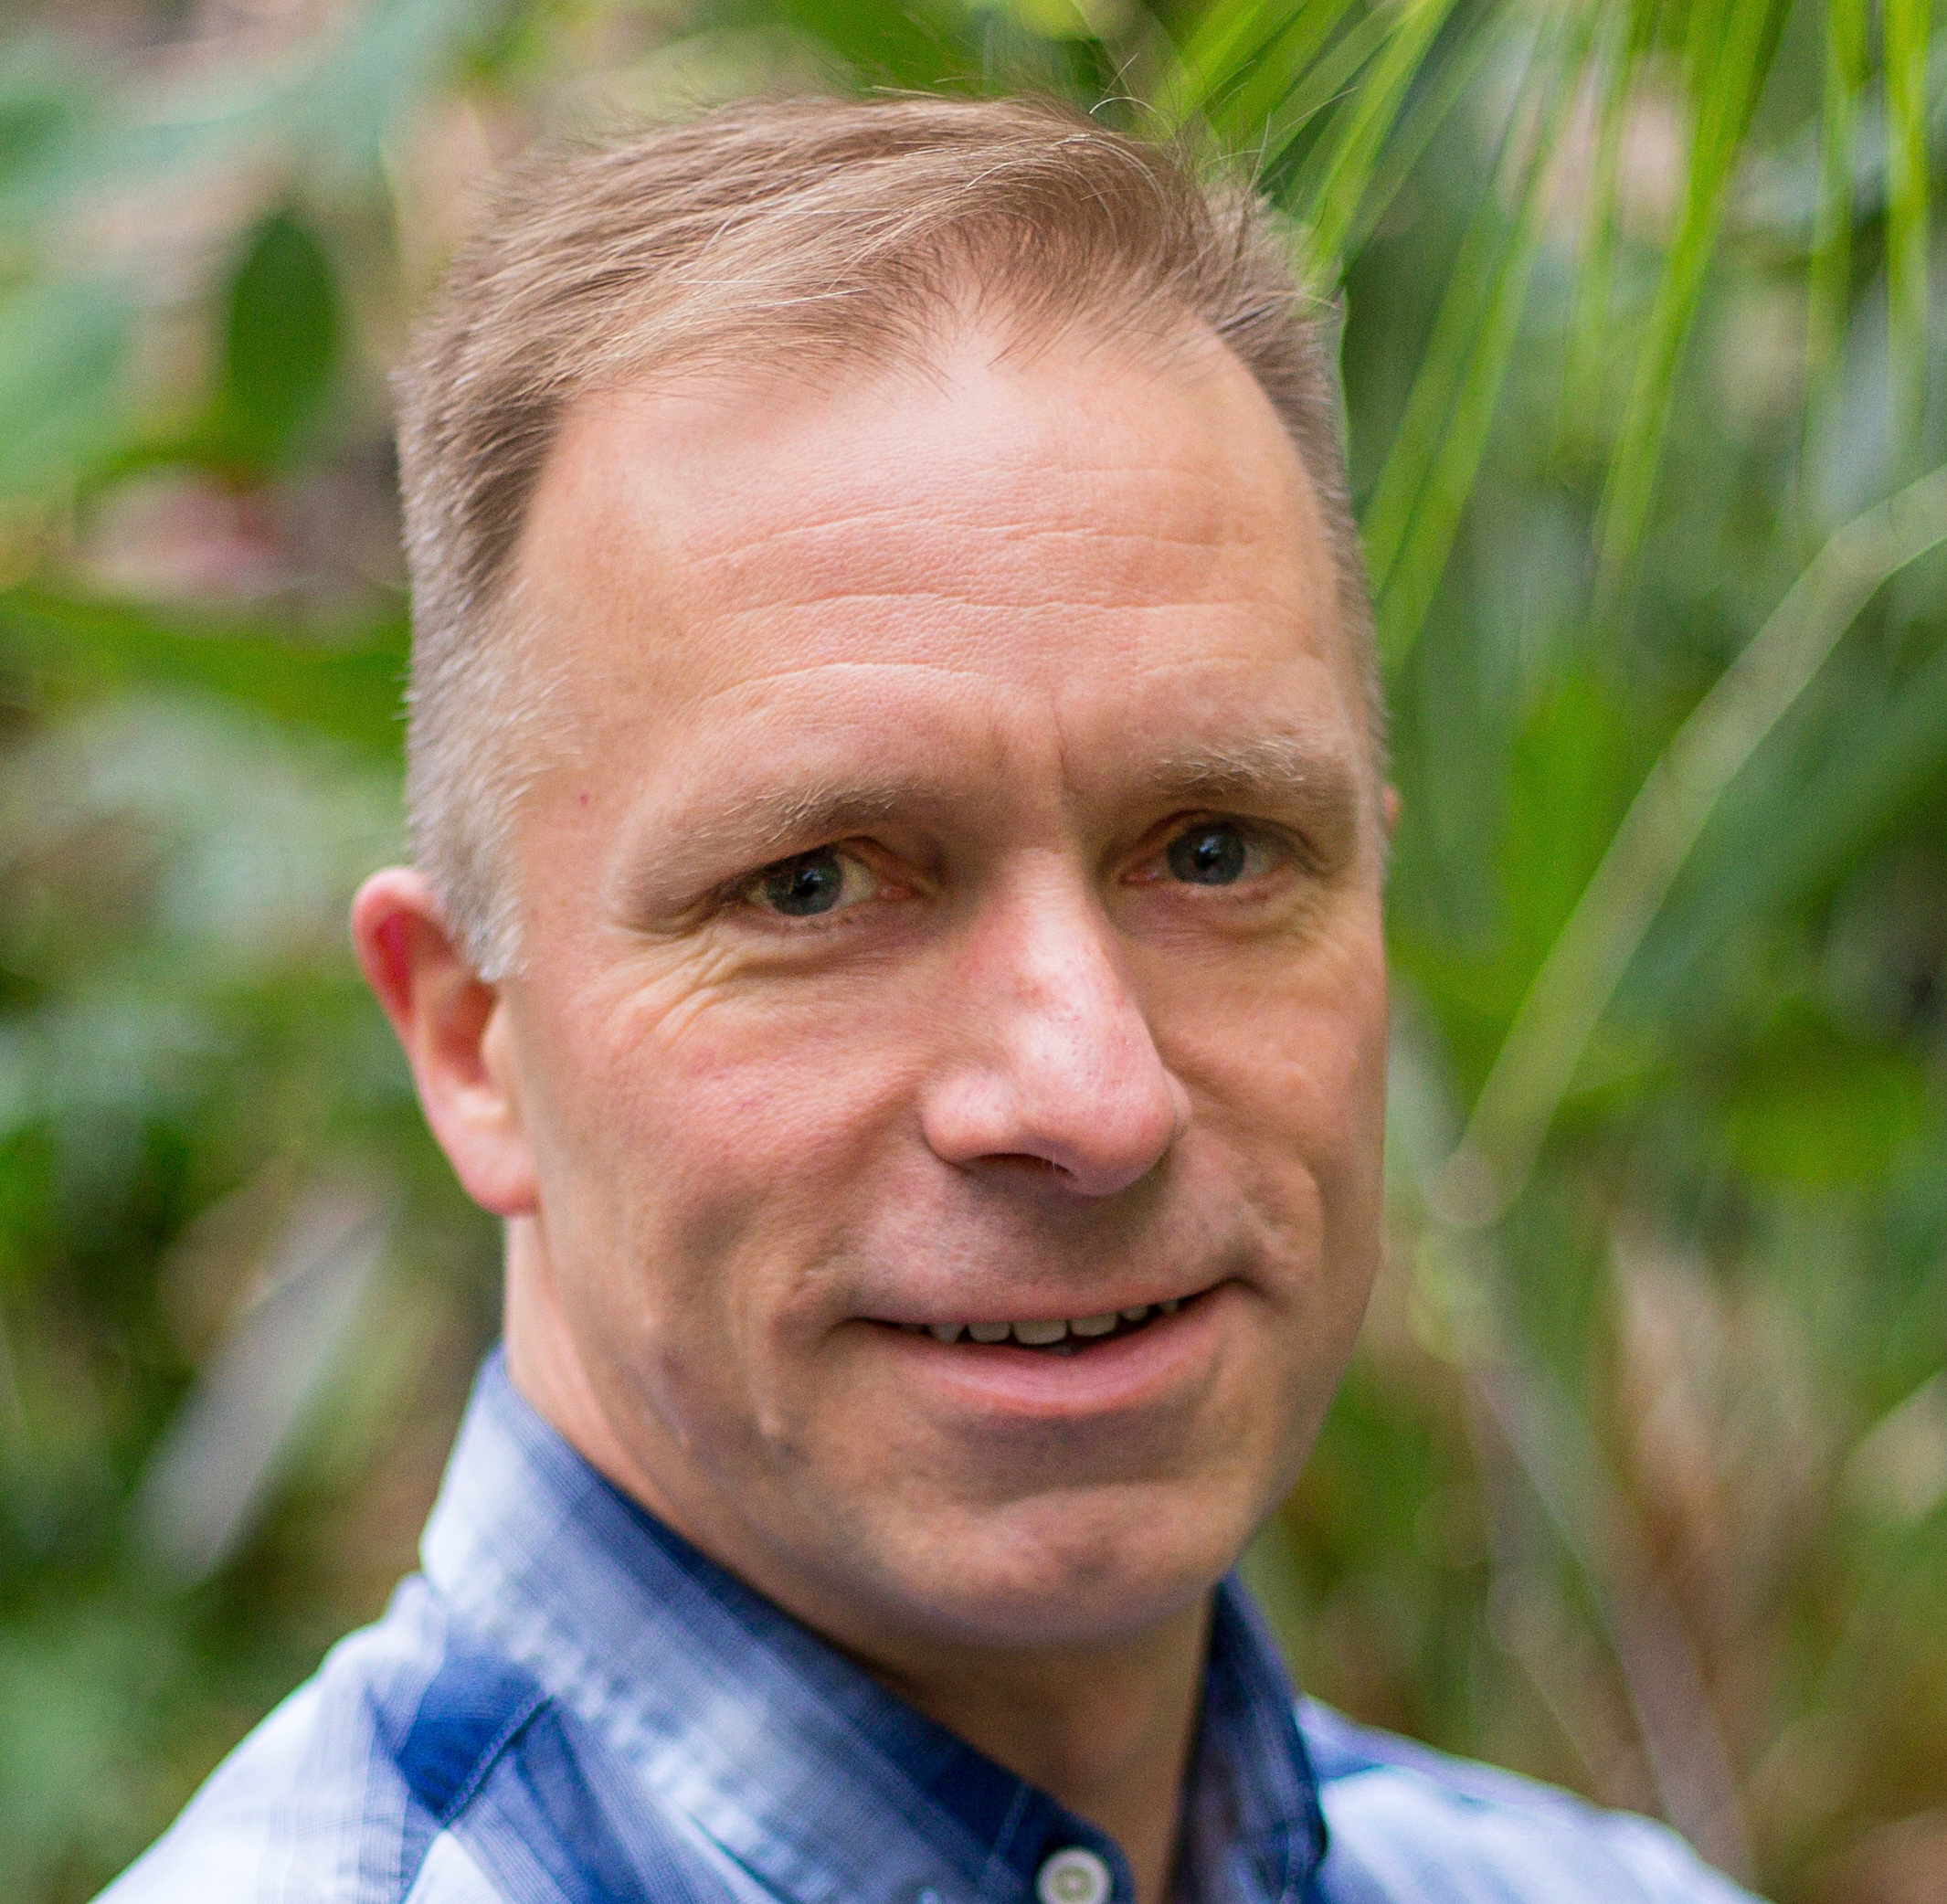
\includegraphics[width=0.25\textwidth]{figures/Heun-pub-photo-headshot}
  \end{center}
\end{wrapfigure}
\textbf{Matthew Kuperus Heun} is Professor of Engineering 
(mechanical concentration)
at Calvin University in Grand Rapids, MI, USA.
He earned an M.S.\ and Ph.D.\ in mechanical engineering from 
the University of Illinois at Urbana-Champaign and 
later worked at NASA's Jet Propulsion Laboratory and at Global Aerospace Corporation. 
He has been a visiting scholar at the Centre for Renewable and Sustainable Energy Studies 
at the University of Stellenbosch, South Africa. 
His long-term research question is 
``What is the relationship between energy and the economy when viewed through the lens of sustainability?''
In addition to scores of articles, he is lead author of 
\emph{Beyond GDP: National accounting in the age of resource depletion}~\citep{Heun:2015aa} 
and a co-editor of
\emph{Beyond Stewardship: New approaches to creation care}~\citep{Warners:2019aa}.
                 % author(s)'s short bio(s)
								% please see the bios folder for some pdf examples
    
    \cleardoublepage

    
% please use TexLive 2014 or later with the M&C macros freely
% available from tug.org or use any other recent version of LaTeX

\documentclass{book}\usepackage[]{graphicx}\usepackage[]{color}
% maxwidth is the original width if it is less than linewidth
% otherwise use linewidth (to make sure the graphics do not exceed the margin)
\makeatletter
\def\maxwidth{ %
  \ifdim\Gin@nat@width>\linewidth
    \linewidth
  \else
    \Gin@nat@width
  \fi
}
\makeatother

\definecolor{fgcolor}{rgb}{0.345, 0.345, 0.345}
\newcommand{\hlnum}[1]{\textcolor[rgb]{0.686,0.059,0.569}{#1}}%
\newcommand{\hlstr}[1]{\textcolor[rgb]{0.192,0.494,0.8}{#1}}%
\newcommand{\hlcom}[1]{\textcolor[rgb]{0.678,0.584,0.686}{\textit{#1}}}%
\newcommand{\hlopt}[1]{\textcolor[rgb]{0,0,0}{#1}}%
\newcommand{\hlstd}[1]{\textcolor[rgb]{0.345,0.345,0.345}{#1}}%
\newcommand{\hlkwa}[1]{\textcolor[rgb]{0.161,0.373,0.58}{\textbf{#1}}}%
\newcommand{\hlkwb}[1]{\textcolor[rgb]{0.69,0.353,0.396}{#1}}%
\newcommand{\hlkwc}[1]{\textcolor[rgb]{0.333,0.667,0.333}{#1}}%
\newcommand{\hlkwd}[1]{\textcolor[rgb]{0.737,0.353,0.396}{\textbf{#1}}}%
\let\hlipl\hlkwb

\usepackage{framed}
\makeatletter
\newenvironment{kframe}{%
 \def\at@end@of@kframe{}%
 \ifinner\ifhmode%
  \def\at@end@of@kframe{\end{minipage}}%
  \begin{minipage}{\columnwidth}%
 \fi\fi%
 \def\FrameCommand##1{\hskip\@totalleftmargin \hskip-\fboxsep
 \colorbox{shadecolor}{##1}\hskip-\fboxsep
     % There is no \\@totalrightmargin, so:
     \hskip-\linewidth \hskip-\@totalleftmargin \hskip\columnwidth}%
 \MakeFramed {\advance\hsize-\width
   \@totalleftmargin\z@ \linewidth\hsize
   \@setminipage}}%
 {\par\unskip\endMakeFramed%
 \at@end@of@kframe}
\makeatother

\definecolor{shadecolor}{rgb}{.97, .97, .97}
\definecolor{messagecolor}{rgb}{0, 0, 0}
\definecolor{warningcolor}{rgb}{1, 0, 1}
\definecolor{errorcolor}{rgb}{1, 0, 0}
\newenvironment{knitrout}{}{} % an empty environment to be redefined in TeX

\usepackage{alltt}

%the main style; default LibreCaslon font
\usepackage[raggedsec]{morgan2}
\usepackage{morgan-defs}

%to use Times New Roman, instead of LibreCaslon, please uncomment the next line
%\morgansetup{fontsetup=times}

% bibliography
% \usepackage[comma,sort,authoryear]{natbib}         % author-year
\usepackage[comma,sort,numbers]{natbib}            % numbered

% Attempting per-chapter bibliographies. Not working yet.
% \usepackage[sectionbib,compress]{natbib}% provides a bibliography for each chapter
% \usepackage{chapterbib}


% 
% Begin LaTeX packages imported by the authors.
% 

\usepackage{booktabs}    % For awesome table formatting
\usepackage[inline]{enumitem}  % For inline enumerate* lists
\usepackage{gensymb}     % For the \degree command
\usepackage{microtype}   % For (more) beautiful typesetting.
\usepackage{rotating}    % For rotating figures.
\usepackage{wrapfig}     % To wrap text around figures.

% 
% Begin LaTeX macros created by the authors.
% 

\newcommand{\degC}{\degree C}

% 
% Begin R and knitr setup
% 






%
% End author additions
% 


\setcounter{secnumdepth}{2}

\graphicspath{{./figures/}}     % folder for the figures in your book

\PassOptionsToPackage{hyphens}{url}
\usepackage[colorlinks=true,linkcolor=MyDarkBlue,
citecolor=MyDarkBlue,filecolor=MyDarkBlue,urlcolor=MyDarkBlue]{hyperref}

\renewcommand{\UrlBreaks}{\do\.\do\@\do\\\do\/\do\!\do\_\do\|\do\;\do\>\do\]%
\do\)\do\,\do\?\do\&\do\'\do+\do\=\do\#%
\do\a\do\b\do\c\do\d\do\e\do\f\do\g\do\h\do\i\do\j%
\do\k\do\l\do\m\do\n\do\o\do\p\do\q\do\r\do\s\do\t%
\do\u\do\v\do\w\do\x\do\y\do\z\do\A\do\B\do\C\do\D%
\do\E\do\F\do\G\do\H\do\I\do\J\do\K\do\L\do\M\do\N%
\do\O\do\P\do\Q\do\R\do\S\do\T\do\U\do\V\do\W\do\X%
\do\Y\do\Z}
\makeatletter
\g@addto@macro{\UrlBreaks}{\UrlOrds}
\renewcommand{\ALG@name}{\color{black}Algorithm}
\makeatother



\makeindex{}                     % if you are creating an index for your book
\IfFileExists{upquote.sty}{\usepackage{upquote}}{}
\begin{document}
% \SweaveOpts{concordance=TRUE}  % Commented on 17 Oct 2019 to eliminate some errors.

 \frontmatter                   % we'll produce the fm for you; 
    
\def\HALFTITLE{The Multifaceted Nature\\
			of Sustainability Challenges:\\
			An Engineering Perspective \\ 
			\textcolor{red}{version $\alpha$ \\}
			\textcolor{black}{\today}}
\def\TITLE{The Multifaceted Nature of Sustainability Challenges\\ 
                        \textcolor{red}{version $\alpha$} \\ \textcolor{black}{\today}}
\def\AUTHORA{Jeremy Van Antwerp}
\def\AFFILIATIONA{Engineering Department, Calvin University}
\def\AUTHORB{Matthew Kuperus Heun}
\def\AFFILIATIONB{Engineering Department, Calvin University}
\def\AUTHORS{\AUTHORA\ and \AUTHORB}
\def\LECTURE{\ \#13}
\def\lcSYNTHESIS{Synthesis Lectures on XYZ}
\def\SYNTHESIS{\MakeUppercase{\textit{\lcSYNTHESIS}}}

\def\EDITOR{xxxx, \textit{yyyy}}


%%%%%%%%%%%% HALF TITLE PAGE 1-2

\thispagestyle{emptyrule}

\halftitle{\HALFTITLE}

\clearpage


%%%%%%%%%%%% FULL TITLE 5

\blankpage

\thispagestyle{emptyrule}
\title{\TITLE}

\vspace*{2pc}
\authorname{\AUTHORA}
\authoraffiliation{\AFFILIATIONA}

\vspace*{1pc}
\authorname{\AUTHORB}
\authoraffiliation{\AFFILIATIONB}

\vfill
\synthesis{\SYNTHESIS\LECTURE}
\morganlogo

\clearpage


%%%%%%%%%%%% ABSTRACT AND KEYWORDS   6

\thispagestyle{emptyrule}

\ABSTRACT
\noindent
The abstract goes here. 

The Abstract and the keywords have to fit in this page.
%end ABSTRACT

\keywords{%
xxx, yyyy, zz
}

\vfill

\clearpage


%%%%%%%%%%%%% DEDICATION  7-8


%{
%\clearpage
%\thispagestyle{plain}
%
%\vspace*{13pc}\Large\it
%\centerline{To Eric, Jacob, and my parents.}
%
%}
%
%\clearpage
 

%%%%%%%%%%%%%%%%%%%%%%%% TOC %%%%%%%%%%%%%%%%%%

%blankpage

{
\pagestyle{plain}
\tableofcontents
}

\clearpage
 
 
%%%%%%%%%%%%%%%%%%%%%%%% PREFACE %%%%%%%%%%%%%%%%%%%
 
 
\blankpage

{
\chapter*{Preface}
\addcontentsline{toc}{chapter}{\protect\numberline{}{Preface}}
\thispagestyle{plain}
\markboth{PREFACE}{PREFACE}

\noindent
\textbf{Who should use this book:} Anyone interested in sustainability. 
This book is intended to be an introduction to the many challenges of 
sustainability and, as such, does not assume any prior background knowledge. \\

\textbf{How to use this book:} Read it. Seriously; that's what you do with books.
This book was written to support a one semester-hour university seminar class
on sustainability. The primary focus of class time is in-class discussion, so 
the end-of-chapter discussion questions should provide about 50\% of the value
in the text. Therefore, individual chapters, or sets of chapters, can easily be
used to support a wide variety of class structures, types, and levels.
Students should read the text on their own, out of class, to get 
basic information related to  the challenges of sustainability. We encourage 
instructors to use a basic and straightforward quiz on the reading through your 
course management platform to hold students accountable for the reading. 
Students should review discussion questions ahead of each class and sketch 
pro and con arguments for each one. \\

\textbf{What you should get out of this book:} This book contains four main 
contributions.
\begin{itemize}
\item Basic facts, figures, and information related to sustainability. We don't 
assume you start with any prior knowledge but by the time you finish reading this
book -- and, by the way, it is easy to read -- you \emph{will} know basic facts
like carbon dioxide concentration in the atmosphere and what are the anthropogenic
sources of carbon dioxide. Furthermore, you should have a \emph{sense of scale}
related to sustainability information. That is, which things are big and 
important and which are smaller and less relavant. To this end, the information
is presented \emph{graphically} as much as possible so that it is easy to see
relative magnitudes.
\item We try to provide an explanatory framework or scaffold thinking about sustainability,
primarily in chapters \ref{chap:introduction}-\ref{chap:carbon_intensity}.
\item The end-of-chapter discussion questions get at moral, ethical, philosophical,
and practical aspects of sustainability. They don't have \sout{right} objective 
answers. Instead, the questions should help illustrate the roll that worldview, 
values, preferences, and \emph{a priori} assumptions have in how we approach sustainability. 
%social pillar?
\item The end-of-chapter project questions range in difficulty from a long
homework problem to a graduate thesis project. If graduate study on a sustainability
topic is in your future, perhaps you can take inspiration from one or more of 
these project questions. Instructors can use one -- or perhaps more -- of these 
questions for a semester-long project, optionally with in-class presentations, for a class.
\end{itemize}
By the end of the book you should see that sustainability is an important, 
urgent, difficult, but solvable problem that requires personal and corporate 
commitments. \\

\textbf{Text organization and schedule.} At one chapter a week, the twelve chapters
in this book don't quite fill a typical university semester. Of course, you don't
have to be in a university context to use this book. A book club or church small group 
are also appropriate audiences -- sustainability is important for everyone. However,
if you are in a university context, here are a few ways that you could fill the 
remaining weeks of your semester. Use class time for project presentations, as
mentioned above. Perhaps groups of students could each be assigned different 
project questions and at the end of the semester, each could share their results.
Alternatively, a class session or sessions could be devoted to a topic or topics your instructor
finds personally interesting, like biofuels, grid-scale storage, or media coverage
of sustainability. At Calvin University, our class devotes a week to worldview
implications for sustainability. You could use our paper \emph{Current disciplines 
and worldviews are insufficient to address sustainability challenges} (2019) as a 
starting place for discussion. % CES website doesn't have 2019 proceedings!
On the other hand, instructors don't need to use all of the book. IEEE Xplore
makes it easy to assign either a single chapter or a group of chapters as supplementary
material for many different types of classes.
Lastly, if you read all the way to the end of the Preface, great job! Give youself a 
gold star. Now, on to the good stuff...


\vspace*{2pc}
\noindent\AUTHORS\\
\noindent December 2021
}

\clearpage


%%%%%%%%%%%%%%%%%%%%%%%% ACK %%%%%%%%%%%%%%%%%%%


\blankpage

\chapter*{Acknowledgments}
\addcontentsline{toc}{chapter}{\protect\numberline{}{Acknowledgments}}
\thispagestyle{plain}
\markboth{ACKNOWLEDGMENTS}{ACKNOWLEDGMENTS}

\noindent
Thanks to the students of the Sustainability Challenges course and our colleague 
Julie Wildschut for teaching the class in fall 2021.

Thanks to research assistants Larisa Tomeci, Henos Tadesse, and Joshua Broekhuisen
for help with sourcing data and creating figures for the text. 
% was there a 4th student?

Thank you to the many reviewers who provided feedback on early versions to the book:
Becky Haney, Jeff Jewett, Shannon Savage, Leonides Murembya, Steve McMullen, Nathan Grawe
Jennifer VanAntwerp, James VanAntwerp, Glen VanAntwerp, Tracy Kuperus, ...

Thanks to the Calvin University Board of Trustees and Joel and Linda Zylstra
for funding to create and revise the text.
Thanks also to Tim Koning of Liquid Haulers Maintenance for funding on biofuels research.



\vspace*{2pc}
\noindent\AUTHORS\\
\noindent December 2021
 
\clearpage

\blankpage

                  % we'll need an Abstract and Keywords
								% please see the abs-pref folder for some pdf examples

 \mainmatter
    % knit_child("chapters/ch01/ch01.Rnw") % \ref{chap:introduction}
    % knit_child("chapters/ch02/ch02.Rnw") % \ref{chap:population}
    % knit_child("chapters/ch03/ch03.Rnw") % \ref{chap:economy}
    % knit_child("chapters/ch04/ch04.Rnw") % \ref{chap:energy}
    % knit_child("chapters/ch05/ch05.Rnw") % \ref{chap:air_and_water}
    % knit_child("chapters/ch06/ch06.Rnw") % \ref{chap:chap:plants_and_animals}
    % knit_child("chapters/ch07/ch07.Rnw") % \ref{chap:food_and_agriculture}
    % knit_child("chapters/ch08/ch08.Rnw") % \ref{chap:transportation}
    % knit_child("chapters/ch09/ch09.Rnw") % \ref{chap:housing_and_households}
    % knit_child("chapters/ch10/ch10.Rnw") % \ref{chap:land_use_and_urban_planning}
    % knit_child("chapters/ch11/ch11.Rnw") % \ref{chap:government_and_regulations} % for tragedy of the commons? https://www.cfra.org/news/131022/water-overcoming-tragedy-commons
    % knit_child("chapters/ch12/ch12.Rnw") % \ref{chap:systems_thinking}
    % knit_child("chapters/ch13/ch13.Rnw") % \ref{chap:values_and_religion}
    % knit_child("chapters/ch14/ch14.Rnw") % \ref{chap:personal_actions}

 %   \input{biblio}              % bibliography

    \bibliographystyle{unsrtnat}
    \bibliography{MCBook2021}   %chktex 11
    
    
    \cleardoublepage

 \backmatter                    % back matter
    
%blankpage

\chapter*{Author's Biography}
\markboth{AUTHOR'S BIOGRAPHY}{AUTHOR'S BIOGRAPHY}
\addcontentsline{toc}{chapter}{\protect\numberline{}{Author's Biography}}


\section*{Jeremy Van Antwerp}

% Adjust spacing so the photo looks nice in the paragraph.
\setlength{\intextsep}{-7pt}%
\setlength{\columnsep}{8pt}%
\begin{wrapfigure}{L}{0.25\textwidth}
  \begin{center}
    \includegraphics[width=0.25\textwidth]{figures/jva-headshot.jpeg}
  \end{center}
\end{wrapfigure}
\textbf{Jeremy Van Antwerp} earned a Ph.D.\ in chemical engineering from 
the University of Illinois at Urbana-Champaign.
More text here.
More text here.
More text here.
More text here.
More text here.
More text here.
More text here.
More text here.
More text here.
More text here.
More text here.
More text here.
More text here.
More text here.
More text here.
More text here.
More text here.
More text here.
More text here.
More text here.
More text here.
More text here.
More text here.
More text here.
More text here.
More text here.
More text here.
More text here.
More text here.
More text here.
More text here.
More text here.
More text here.
More text here.
More text here.
More text here.
More text here.
More text here.
More text here.
More text here.
More text here.
More text here.
More text here.
More text here.
More text here.
More text here.
More text here.
More text here.
More text here.


\section*{Matthew Kuperus Heun}

% Adjust spacing so the photo looks nice in the paragraph.
\setlength{\intextsep}{-7pt}%
\setlength{\columnsep}{8pt}%
\begin{wrapfigure}{L}{0.25\textwidth}
  \begin{center}
    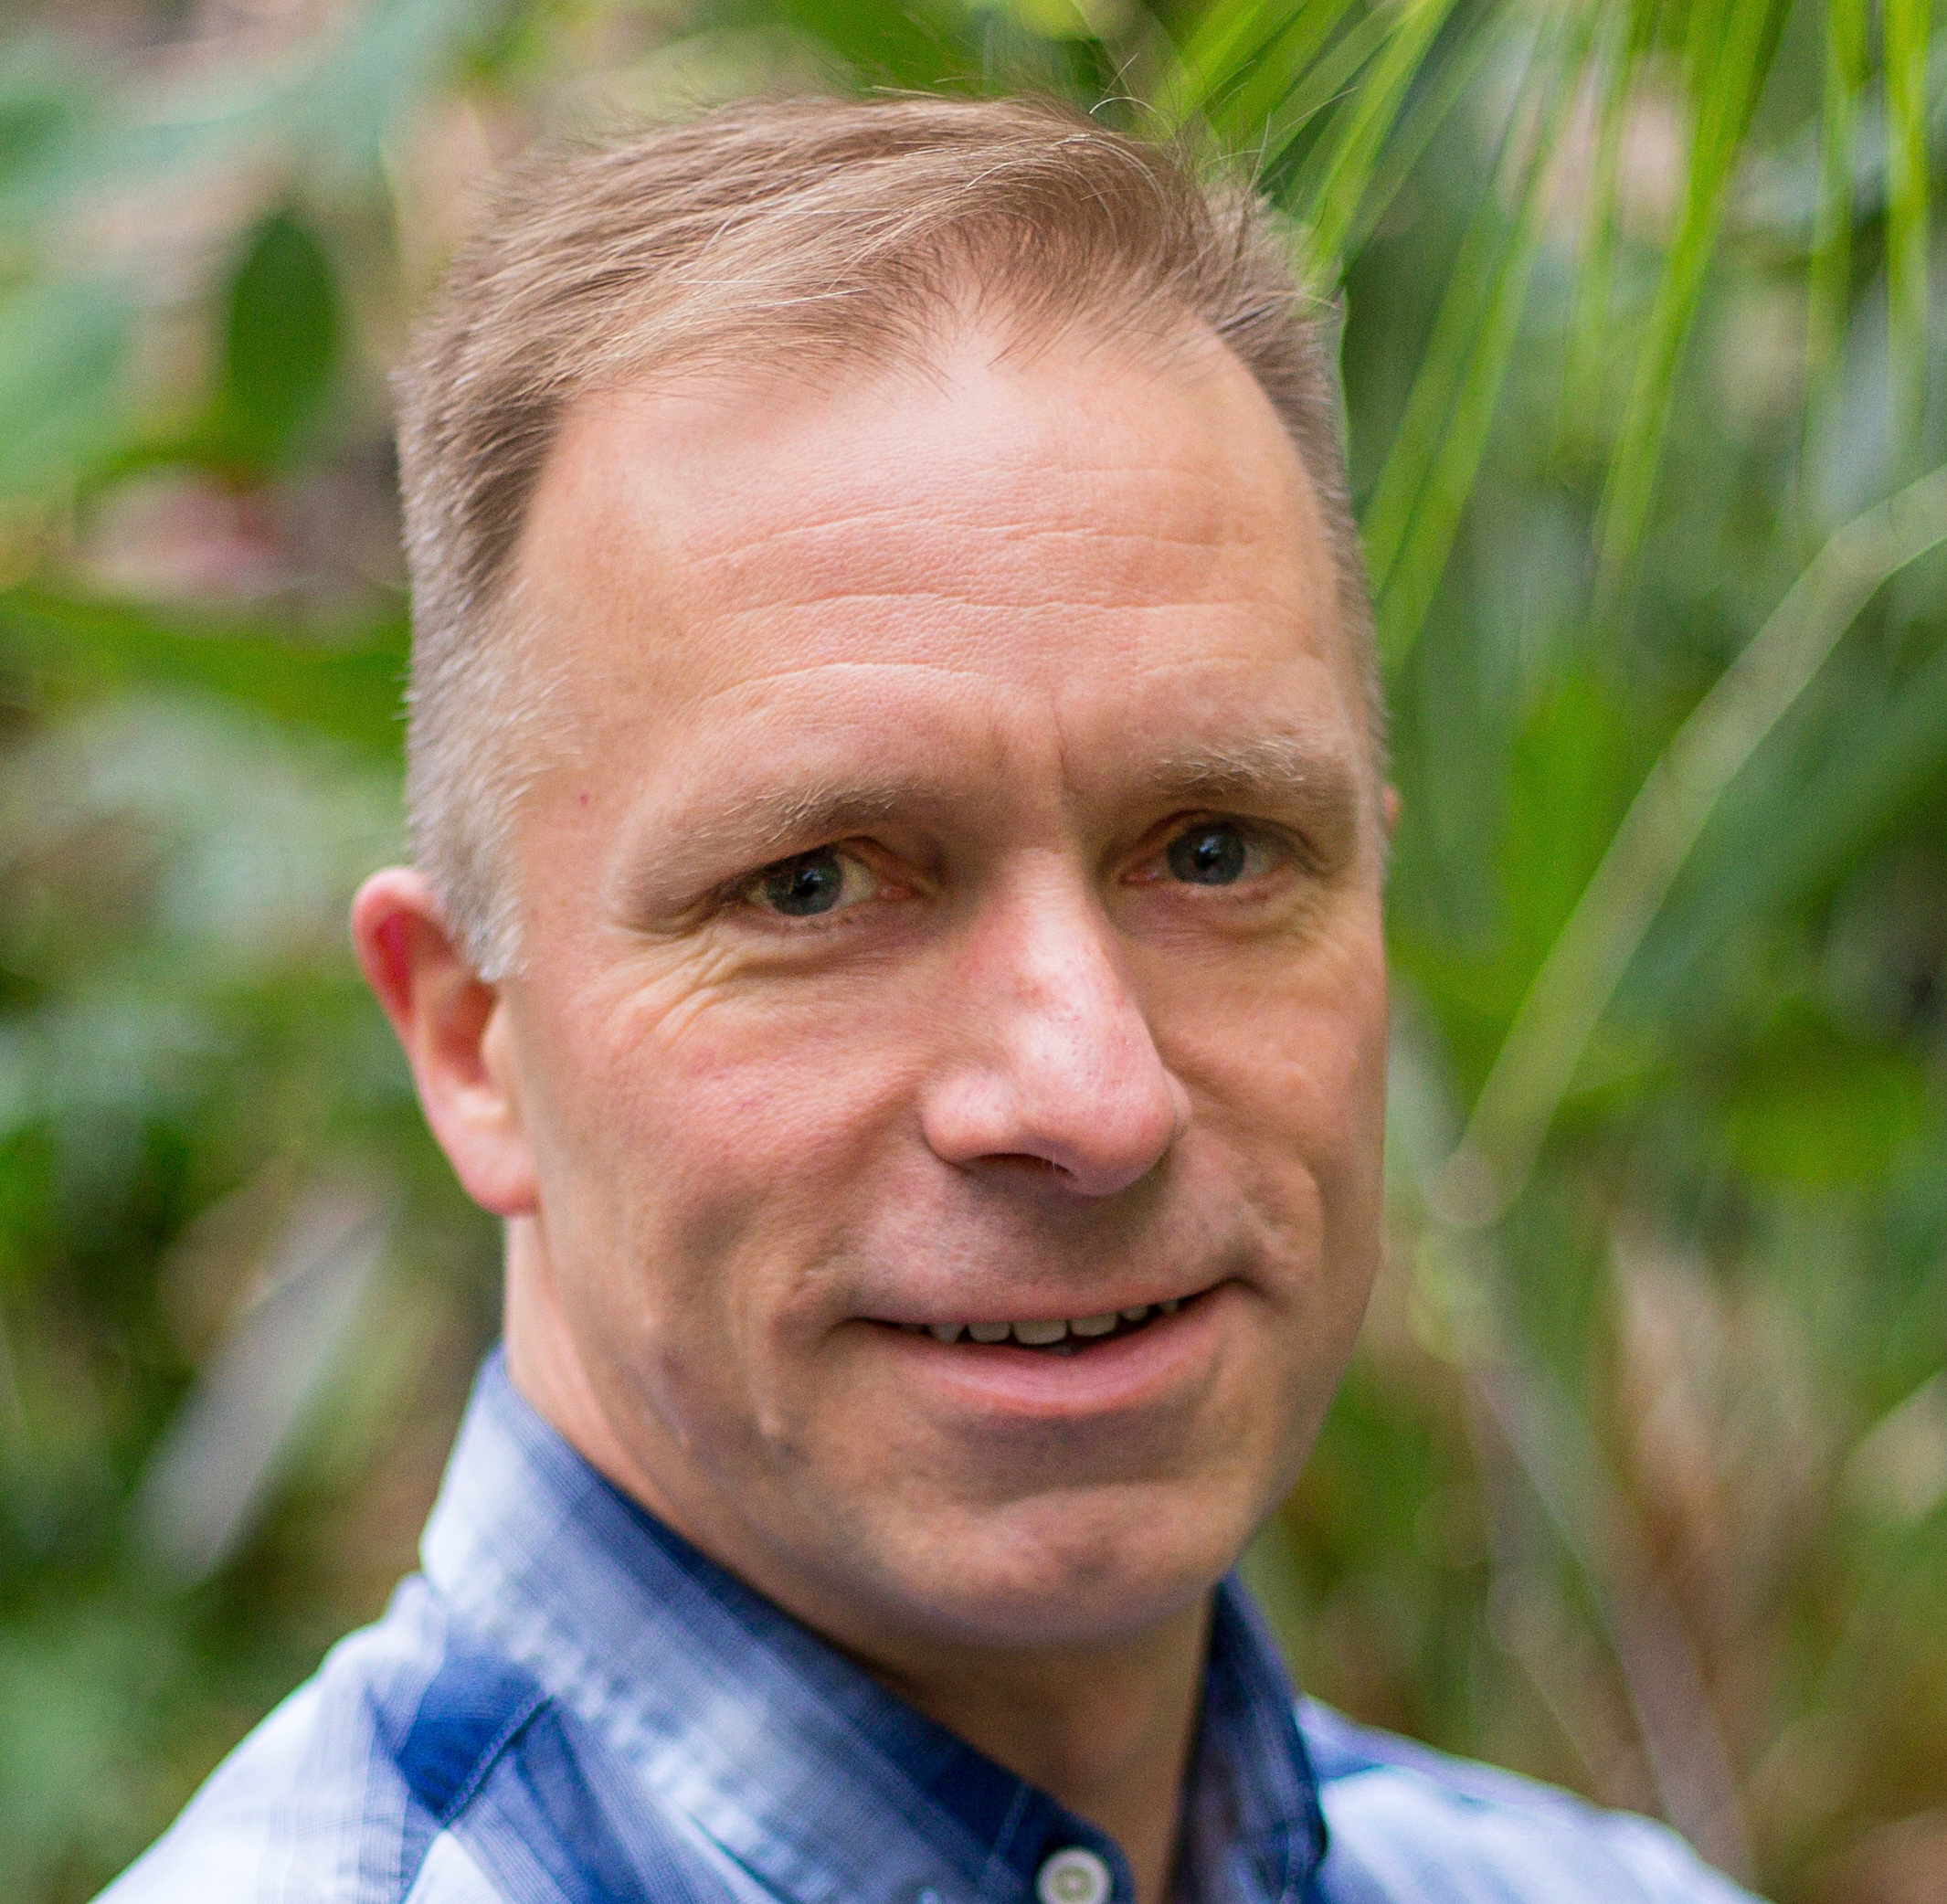
\includegraphics[width=0.25\textwidth]{figures/Heun-pub-photo-headshot}
  \end{center}
\end{wrapfigure}
\textbf{Matthew Kuperus Heun} is Professor of Engineering 
(mechanical concentration)
at Calvin University in Grand Rapids, MI, USA.
He earned an M.S.\ and Ph.D.\ in mechanical engineering from 
the University of Illinois at Urbana-Champaign and 
later worked at NASA's Jet Propulsion Laboratory and at Global Aerospace Corporation. 
He has been a visiting scholar at the Centre for Renewable and Sustainable Energy Studies 
at the University of Stellenbosch, South Africa. 
His long-term research question is 
``What is the relationship between energy and the economy when viewed through the lens of sustainability?''
In addition to scores of articles, he is lead author of 
\emph{Beyond GDP: National accounting in the age of resource depletion}~\citep{Heun:2015aa} 
and a co-editor of
\emph{Beyond Stewardship: New approaches to creation care}~\citep{Warners:2019aa}.
                 % author(s)'s short bio(s)
								% please see the bios folder for some pdf examples
    
    \cleardoublepage

    
% please use TexLive 2014 or later with the M&C macros freely
% available from tug.org or use any other recent version of LaTeX

\documentclass{book}\usepackage[]{graphicx}\usepackage[]{color}
% maxwidth is the original width if it is less than linewidth
% otherwise use linewidth (to make sure the graphics do not exceed the margin)
\makeatletter
\def\maxwidth{ %
  \ifdim\Gin@nat@width>\linewidth
    \linewidth
  \else
    \Gin@nat@width
  \fi
}
\makeatother

\definecolor{fgcolor}{rgb}{0.345, 0.345, 0.345}
\newcommand{\hlnum}[1]{\textcolor[rgb]{0.686,0.059,0.569}{#1}}%
\newcommand{\hlstr}[1]{\textcolor[rgb]{0.192,0.494,0.8}{#1}}%
\newcommand{\hlcom}[1]{\textcolor[rgb]{0.678,0.584,0.686}{\textit{#1}}}%
\newcommand{\hlopt}[1]{\textcolor[rgb]{0,0,0}{#1}}%
\newcommand{\hlstd}[1]{\textcolor[rgb]{0.345,0.345,0.345}{#1}}%
\newcommand{\hlkwa}[1]{\textcolor[rgb]{0.161,0.373,0.58}{\textbf{#1}}}%
\newcommand{\hlkwb}[1]{\textcolor[rgb]{0.69,0.353,0.396}{#1}}%
\newcommand{\hlkwc}[1]{\textcolor[rgb]{0.333,0.667,0.333}{#1}}%
\newcommand{\hlkwd}[1]{\textcolor[rgb]{0.737,0.353,0.396}{\textbf{#1}}}%
\let\hlipl\hlkwb

\usepackage{framed}
\makeatletter
\newenvironment{kframe}{%
 \def\at@end@of@kframe{}%
 \ifinner\ifhmode%
  \def\at@end@of@kframe{\end{minipage}}%
  \begin{minipage}{\columnwidth}%
 \fi\fi%
 \def\FrameCommand##1{\hskip\@totalleftmargin \hskip-\fboxsep
 \colorbox{shadecolor}{##1}\hskip-\fboxsep
     % There is no \\@totalrightmargin, so:
     \hskip-\linewidth \hskip-\@totalleftmargin \hskip\columnwidth}%
 \MakeFramed {\advance\hsize-\width
   \@totalleftmargin\z@ \linewidth\hsize
   \@setminipage}}%
 {\par\unskip\endMakeFramed%
 \at@end@of@kframe}
\makeatother

\definecolor{shadecolor}{rgb}{.97, .97, .97}
\definecolor{messagecolor}{rgb}{0, 0, 0}
\definecolor{warningcolor}{rgb}{1, 0, 1}
\definecolor{errorcolor}{rgb}{1, 0, 0}
\newenvironment{knitrout}{}{} % an empty environment to be redefined in TeX

\usepackage{alltt}

%the main style; default LibreCaslon font
\usepackage[raggedsec]{morgan2}
\usepackage{morgan-defs}

%to use Times New Roman, instead of LibreCaslon, please uncomment the next line
%\morgansetup{fontsetup=times}

% bibliography
% \usepackage[comma,sort,authoryear]{natbib}         % author-year
\usepackage[comma,sort,numbers]{natbib}            % numbered

% Attempting per-chapter bibliographies. Not working yet.
% \usepackage[sectionbib,compress]{natbib}% provides a bibliography for each chapter
% \usepackage{chapterbib}


% 
% Begin LaTeX packages imported by the authors.
% 

\usepackage{booktabs}    % For awesome table formatting
\usepackage[inline]{enumitem}  % For inline enumerate* lists
\usepackage{gensymb}     % For the \degree command
\usepackage{microtype}   % For (more) beautiful typesetting.
\usepackage{rotating}    % For rotating figures.
\usepackage{wrapfig}     % To wrap text around figures.

% 
% Begin LaTeX macros created by the authors.
% 

\newcommand{\degC}{\degree C}

% 
% Begin R and knitr setup
% 






%
% End author additions
% 


\setcounter{secnumdepth}{2}

\graphicspath{{./figures/}}     % folder for the figures in your book

\PassOptionsToPackage{hyphens}{url}
\usepackage[colorlinks=true,linkcolor=MyDarkBlue,
citecolor=MyDarkBlue,filecolor=MyDarkBlue,urlcolor=MyDarkBlue]{hyperref}

\renewcommand{\UrlBreaks}{\do\.\do\@\do\\\do\/\do\!\do\_\do\|\do\;\do\>\do\]%
\do\)\do\,\do\?\do\&\do\'\do+\do\=\do\#%
\do\a\do\b\do\c\do\d\do\e\do\f\do\g\do\h\do\i\do\j%
\do\k\do\l\do\m\do\n\do\o\do\p\do\q\do\r\do\s\do\t%
\do\u\do\v\do\w\do\x\do\y\do\z\do\A\do\B\do\C\do\D%
\do\E\do\F\do\G\do\H\do\I\do\J\do\K\do\L\do\M\do\N%
\do\O\do\P\do\Q\do\R\do\S\do\T\do\U\do\V\do\W\do\X%
\do\Y\do\Z}
\makeatletter
\g@addto@macro{\UrlBreaks}{\UrlOrds}
\renewcommand{\ALG@name}{\color{black}Algorithm}
\makeatother



\makeindex{}                     % if you are creating an index for your book
\IfFileExists{upquote.sty}{\usepackage{upquote}}{}
\begin{document}
% \SweaveOpts{concordance=TRUE}  % Commented on 17 Oct 2019 to eliminate some errors.

 \frontmatter                   % we'll produce the fm for you; 
    
\def\HALFTITLE{The Multifaceted Nature\\
			of Sustainability Challenges:\\
			An Engineering Perspective \\ 
			\textcolor{red}{version $\alpha$ \\}
			\textcolor{black}{\today}}
\def\TITLE{The Multifaceted Nature of Sustainability Challenges\\ 
                        \textcolor{red}{version $\alpha$} \\ \textcolor{black}{\today}}
\def\AUTHORA{Jeremy Van Antwerp}
\def\AFFILIATIONA{Engineering Department, Calvin University}
\def\AUTHORB{Matthew Kuperus Heun}
\def\AFFILIATIONB{Engineering Department, Calvin University}
\def\AUTHORS{\AUTHORA\ and \AUTHORB}
\def\LECTURE{\ \#13}
\def\lcSYNTHESIS{Synthesis Lectures on XYZ}
\def\SYNTHESIS{\MakeUppercase{\textit{\lcSYNTHESIS}}}

\def\EDITOR{xxxx, \textit{yyyy}}


%%%%%%%%%%%% HALF TITLE PAGE 1-2

\thispagestyle{emptyrule}

\halftitle{\HALFTITLE}

\clearpage


%%%%%%%%%%%% FULL TITLE 5

\blankpage

\thispagestyle{emptyrule}
\title{\TITLE}

\vspace*{2pc}
\authorname{\AUTHORA}
\authoraffiliation{\AFFILIATIONA}

\vspace*{1pc}
\authorname{\AUTHORB}
\authoraffiliation{\AFFILIATIONB}

\vfill
\synthesis{\SYNTHESIS\LECTURE}
\morganlogo

\clearpage


%%%%%%%%%%%% ABSTRACT AND KEYWORDS   6

\thispagestyle{emptyrule}

\ABSTRACT
\noindent
The abstract goes here. 

The Abstract and the keywords have to fit in this page.
%end ABSTRACT

\keywords{%
xxx, yyyy, zz
}

\vfill

\clearpage


%%%%%%%%%%%%% DEDICATION  7-8


%{
%\clearpage
%\thispagestyle{plain}
%
%\vspace*{13pc}\Large\it
%\centerline{To Eric, Jacob, and my parents.}
%
%}
%
%\clearpage
 

%%%%%%%%%%%%%%%%%%%%%%%% TOC %%%%%%%%%%%%%%%%%%

%blankpage

{
\pagestyle{plain}
\tableofcontents
}

\clearpage
 
 
%%%%%%%%%%%%%%%%%%%%%%%% PREFACE %%%%%%%%%%%%%%%%%%%
 
 
\blankpage

{
\chapter*{Preface}
\addcontentsline{toc}{chapter}{\protect\numberline{}{Preface}}
\thispagestyle{plain}
\markboth{PREFACE}{PREFACE}

\noindent
\textbf{Who should use this book:} Anyone interested in sustainability. 
This book is intended to be an introduction to the many challenges of 
sustainability and, as such, does not assume any prior background knowledge. \\

\textbf{How to use this book:} Read it. Seriously; that's what you do with books.
This book was written to support a one semester-hour university seminar class
on sustainability. The primary focus of class time is in-class discussion, so 
the end-of-chapter discussion questions should provide about 50\% of the value
in the text. Therefore, individual chapters, or sets of chapters, can easily be
used to support a wide variety of class structures, types, and levels.
Students should read the text on their own, out of class, to get 
basic information related to  the challenges of sustainability. We encourage 
instructors to use a basic and straightforward quiz on the reading through your 
course management platform to hold students accountable for the reading. 
Students should review discussion questions ahead of each class and sketch 
pro and con arguments for each one. \\

\textbf{What you should get out of this book:} This book contains four main 
contributions.
\begin{itemize}
\item Basic facts, figures, and information related to sustainability. We don't 
assume you start with any prior knowledge but by the time you finish reading this
book -- and, by the way, it is easy to read -- you \emph{will} know basic facts
like carbon dioxide concentration in the atmosphere and what are the anthropogenic
sources of carbon dioxide. Furthermore, you should have a \emph{sense of scale}
related to sustainability information. That is, which things are big and 
important and which are smaller and less relavant. To this end, the information
is presented \emph{graphically} as much as possible so that it is easy to see
relative magnitudes.
\item We try to provide an explanatory framework or scaffold thinking about sustainability,
primarily in chapters \ref{chap:introduction}-\ref{chap:carbon_intensity}.
\item The end-of-chapter discussion questions get at moral, ethical, philosophical,
and practical aspects of sustainability. They don't have \sout{right} objective 
answers. Instead, the questions should help illustrate the roll that worldview, 
values, preferences, and \emph{a priori} assumptions have in how we approach sustainability. 
%social pillar?
\item The end-of-chapter project questions range in difficulty from a long
homework problem to a graduate thesis project. If graduate study on a sustainability
topic is in your future, perhaps you can take inspiration from one or more of 
these project questions. Instructors can use one -- or perhaps more -- of these 
questions for a semester-long project, optionally with in-class presentations, for a class.
\end{itemize}
By the end of the book you should see that sustainability is an important, 
urgent, difficult, but solvable problem that requires personal and corporate 
commitments. \\

\textbf{Text organization and schedule.} At one chapter a week, the twelve chapters
in this book don't quite fill a typical university semester. Of course, you don't
have to be in a university context to use this book. A book club or church small group 
are also appropriate audiences -- sustainability is important for everyone. However,
if you are in a university context, here are a few ways that you could fill the 
remaining weeks of your semester. Use class time for project presentations, as
mentioned above. Perhaps groups of students could each be assigned different 
project questions and at the end of the semester, each could share their results.
Alternatively, a class session or sessions could be devoted to a topic or topics your instructor
finds personally interesting, like biofuels, grid-scale storage, or media coverage
of sustainability. At Calvin University, our class devotes a week to worldview
implications for sustainability. You could use our paper \emph{Current disciplines 
and worldviews are insufficient to address sustainability challenges} (2019) as a 
starting place for discussion. % CES website doesn't have 2019 proceedings!
On the other hand, instructors don't need to use all of the book. IEEE Xplore
makes it easy to assign either a single chapter or a group of chapters as supplementary
material for many different types of classes.
Lastly, if you read all the way to the end of the Preface, great job! Give youself a 
gold star. Now, on to the good stuff...


\vspace*{2pc}
\noindent\AUTHORS\\
\noindent December 2021
}

\clearpage


%%%%%%%%%%%%%%%%%%%%%%%% ACK %%%%%%%%%%%%%%%%%%%


\blankpage

\chapter*{Acknowledgments}
\addcontentsline{toc}{chapter}{\protect\numberline{}{Acknowledgments}}
\thispagestyle{plain}
\markboth{ACKNOWLEDGMENTS}{ACKNOWLEDGMENTS}

\noindent
Thanks to the students of the Sustainability Challenges course and our colleague 
Julie Wildschut for teaching the class in fall 2021.

Thanks to research assistants Larisa Tomeci, Henos Tadesse, and Joshua Broekhuisen
for help with sourcing data and creating figures for the text. 
% was there a 4th student?

Thank you to the many reviewers who provided feedback on early versions to the book:
Becky Haney, Jeff Jewett, Shannon Savage, Leonides Murembya, Steve McMullen, Nathan Grawe
Jennifer VanAntwerp, James VanAntwerp, Glen VanAntwerp, Tracy Kuperus, ...

Thanks to the Calvin University Board of Trustees and Joel and Linda Zylstra
for funding to create and revise the text.
Thanks also to Tim Koning of Liquid Haulers Maintenance for funding on biofuels research.



\vspace*{2pc}
\noindent\AUTHORS\\
\noindent December 2021
 
\clearpage

\blankpage

                  % we'll need an Abstract and Keywords
								% please see the abs-pref folder for some pdf examples

 \mainmatter
    % knit_child("chapters/ch01/ch01.Rnw") % \ref{chap:introduction}
    % knit_child("chapters/ch02/ch02.Rnw") % \ref{chap:population}
    % knit_child("chapters/ch03/ch03.Rnw") % \ref{chap:economy}
    % knit_child("chapters/ch04/ch04.Rnw") % \ref{chap:energy}
    % knit_child("chapters/ch05/ch05.Rnw") % \ref{chap:air_and_water}
    % knit_child("chapters/ch06/ch06.Rnw") % \ref{chap:chap:plants_and_animals}
    % knit_child("chapters/ch07/ch07.Rnw") % \ref{chap:food_and_agriculture}
    % knit_child("chapters/ch08/ch08.Rnw") % \ref{chap:transportation}
    % knit_child("chapters/ch09/ch09.Rnw") % \ref{chap:housing_and_households}
    % knit_child("chapters/ch10/ch10.Rnw") % \ref{chap:land_use_and_urban_planning}
    % knit_child("chapters/ch11/ch11.Rnw") % \ref{chap:government_and_regulations} % for tragedy of the commons? https://www.cfra.org/news/131022/water-overcoming-tragedy-commons
    % knit_child("chapters/ch12/ch12.Rnw") % \ref{chap:systems_thinking}
    % knit_child("chapters/ch13/ch13.Rnw") % \ref{chap:values_and_religion}
    % knit_child("chapters/ch14/ch14.Rnw") % \ref{chap:personal_actions}

 %   \input{biblio}              % bibliography

    \bibliographystyle{unsrtnat}
    \bibliography{MCBook2021}   %chktex 11
    
    
    \cleardoublepage

 \backmatter                    % back matter
    
%blankpage

\chapter*{Author's Biography}
\markboth{AUTHOR'S BIOGRAPHY}{AUTHOR'S BIOGRAPHY}
\addcontentsline{toc}{chapter}{\protect\numberline{}{Author's Biography}}


\section*{Jeremy Van Antwerp}

% Adjust spacing so the photo looks nice in the paragraph.
\setlength{\intextsep}{-7pt}%
\setlength{\columnsep}{8pt}%
\begin{wrapfigure}{L}{0.25\textwidth}
  \begin{center}
    \includegraphics[width=0.25\textwidth]{figures/jva-headshot.jpeg}
  \end{center}
\end{wrapfigure}
\textbf{Jeremy Van Antwerp} earned a Ph.D.\ in chemical engineering from 
the University of Illinois at Urbana-Champaign.
More text here.
More text here.
More text here.
More text here.
More text here.
More text here.
More text here.
More text here.
More text here.
More text here.
More text here.
More text here.
More text here.
More text here.
More text here.
More text here.
More text here.
More text here.
More text here.
More text here.
More text here.
More text here.
More text here.
More text here.
More text here.
More text here.
More text here.
More text here.
More text here.
More text here.
More text here.
More text here.
More text here.
More text here.
More text here.
More text here.
More text here.
More text here.
More text here.
More text here.
More text here.
More text here.
More text here.
More text here.
More text here.
More text here.
More text here.
More text here.
More text here.


\section*{Matthew Kuperus Heun}

% Adjust spacing so the photo looks nice in the paragraph.
\setlength{\intextsep}{-7pt}%
\setlength{\columnsep}{8pt}%
\begin{wrapfigure}{L}{0.25\textwidth}
  \begin{center}
    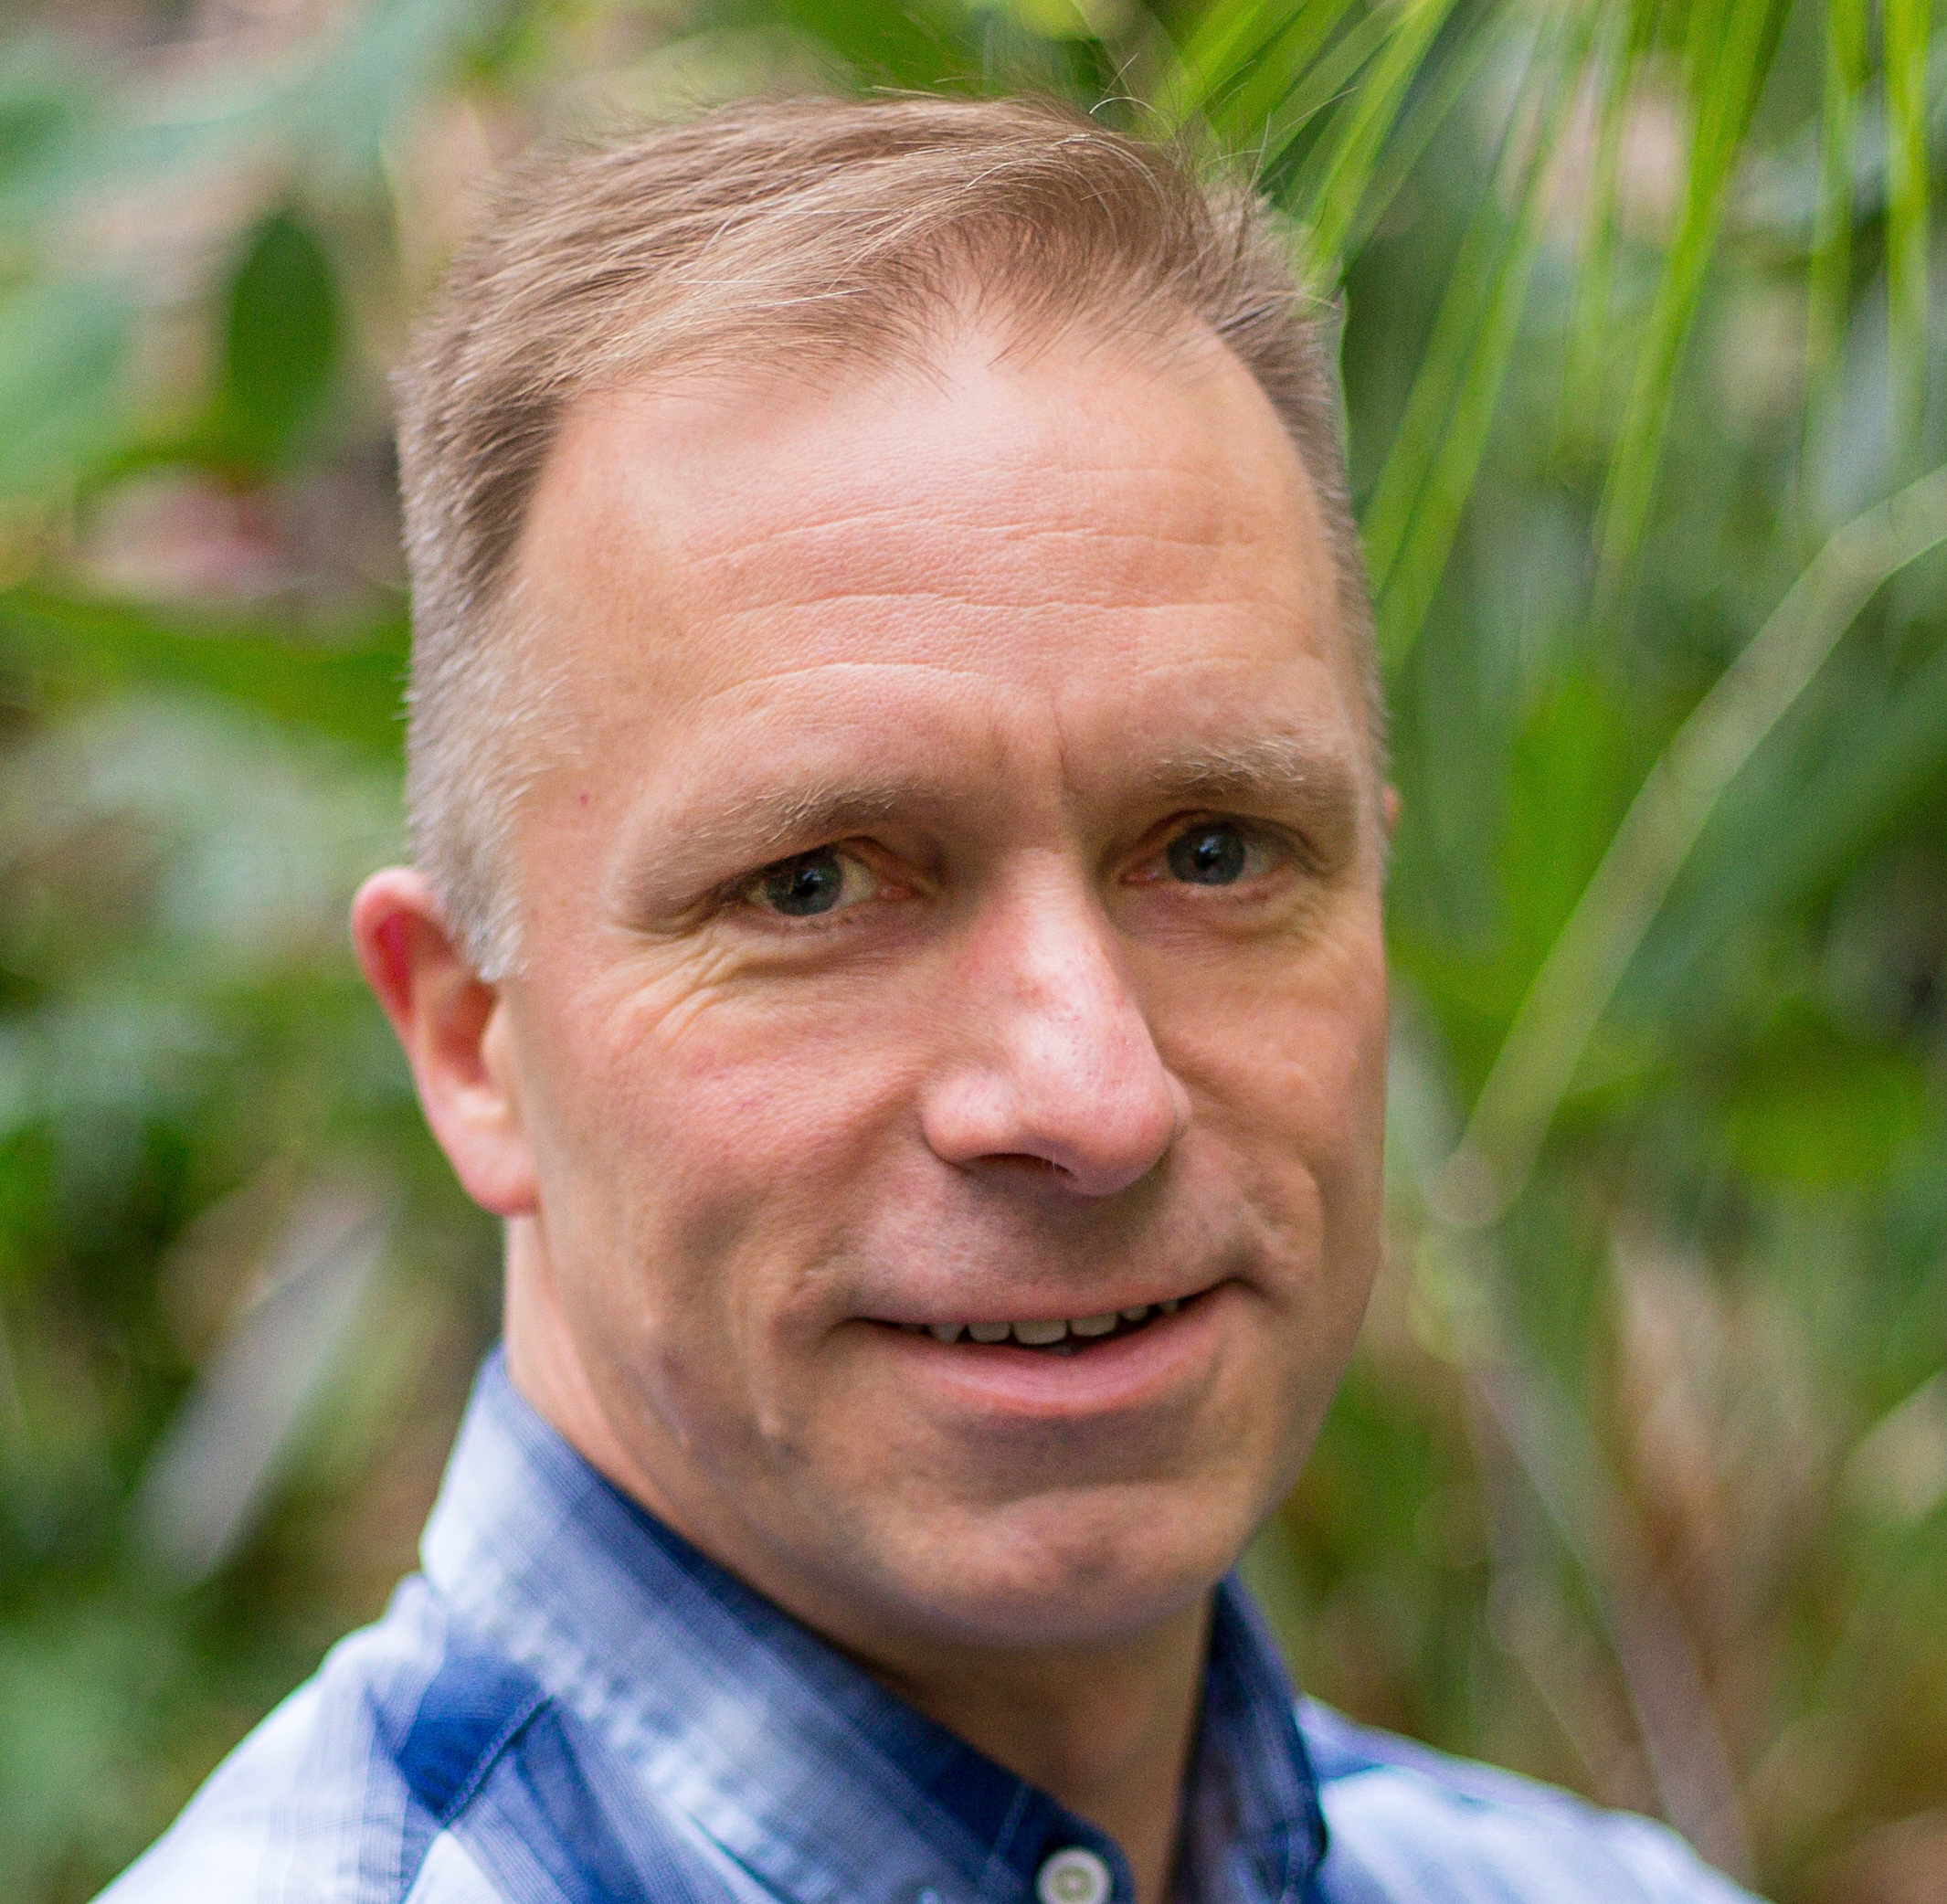
\includegraphics[width=0.25\textwidth]{figures/Heun-pub-photo-headshot}
  \end{center}
\end{wrapfigure}
\textbf{Matthew Kuperus Heun} is Professor of Engineering 
(mechanical concentration)
at Calvin University in Grand Rapids, MI, USA.
He earned an M.S.\ and Ph.D.\ in mechanical engineering from 
the University of Illinois at Urbana-Champaign and 
later worked at NASA's Jet Propulsion Laboratory and at Global Aerospace Corporation. 
He has been a visiting scholar at the Centre for Renewable and Sustainable Energy Studies 
at the University of Stellenbosch, South Africa. 
His long-term research question is 
``What is the relationship between energy and the economy when viewed through the lens of sustainability?''
In addition to scores of articles, he is lead author of 
\emph{Beyond GDP: National accounting in the age of resource depletion}~\citep{Heun:2015aa} 
and a co-editor of
\emph{Beyond Stewardship: New approaches to creation care}~\citep{Warners:2019aa}.
                 % author(s)'s short bio(s)
								% please see the bios folder for some pdf examples
    
    \cleardoublepage

    
% please use TexLive 2014 or later with the M&C macros freely
% available from tug.org or use any other recent version of LaTeX

\documentclass{book}\usepackage[]{graphicx}\usepackage[]{color}
% maxwidth is the original width if it is less than linewidth
% otherwise use linewidth (to make sure the graphics do not exceed the margin)
\makeatletter
\def\maxwidth{ %
  \ifdim\Gin@nat@width>\linewidth
    \linewidth
  \else
    \Gin@nat@width
  \fi
}
\makeatother

\definecolor{fgcolor}{rgb}{0.345, 0.345, 0.345}
\newcommand{\hlnum}[1]{\textcolor[rgb]{0.686,0.059,0.569}{#1}}%
\newcommand{\hlstr}[1]{\textcolor[rgb]{0.192,0.494,0.8}{#1}}%
\newcommand{\hlcom}[1]{\textcolor[rgb]{0.678,0.584,0.686}{\textit{#1}}}%
\newcommand{\hlopt}[1]{\textcolor[rgb]{0,0,0}{#1}}%
\newcommand{\hlstd}[1]{\textcolor[rgb]{0.345,0.345,0.345}{#1}}%
\newcommand{\hlkwa}[1]{\textcolor[rgb]{0.161,0.373,0.58}{\textbf{#1}}}%
\newcommand{\hlkwb}[1]{\textcolor[rgb]{0.69,0.353,0.396}{#1}}%
\newcommand{\hlkwc}[1]{\textcolor[rgb]{0.333,0.667,0.333}{#1}}%
\newcommand{\hlkwd}[1]{\textcolor[rgb]{0.737,0.353,0.396}{\textbf{#1}}}%
\let\hlipl\hlkwb

\usepackage{framed}
\makeatletter
\newenvironment{kframe}{%
 \def\at@end@of@kframe{}%
 \ifinner\ifhmode%
  \def\at@end@of@kframe{\end{minipage}}%
  \begin{minipage}{\columnwidth}%
 \fi\fi%
 \def\FrameCommand##1{\hskip\@totalleftmargin \hskip-\fboxsep
 \colorbox{shadecolor}{##1}\hskip-\fboxsep
     % There is no \\@totalrightmargin, so:
     \hskip-\linewidth \hskip-\@totalleftmargin \hskip\columnwidth}%
 \MakeFramed {\advance\hsize-\width
   \@totalleftmargin\z@ \linewidth\hsize
   \@setminipage}}%
 {\par\unskip\endMakeFramed%
 \at@end@of@kframe}
\makeatother

\definecolor{shadecolor}{rgb}{.97, .97, .97}
\definecolor{messagecolor}{rgb}{0, 0, 0}
\definecolor{warningcolor}{rgb}{1, 0, 1}
\definecolor{errorcolor}{rgb}{1, 0, 0}
\newenvironment{knitrout}{}{} % an empty environment to be redefined in TeX

\usepackage{alltt}

%the main style; default LibreCaslon font
\usepackage[raggedsec]{morgan2}
\usepackage{morgan-defs}

%to use Times New Roman, instead of LibreCaslon, please uncomment the next line
%\morgansetup{fontsetup=times}

% bibliography
% \usepackage[comma,sort,authoryear]{natbib}         % author-year
\usepackage[comma,sort,numbers]{natbib}            % numbered

% Attempting per-chapter bibliographies. Not working yet.
% \usepackage[sectionbib,compress]{natbib}% provides a bibliography for each chapter
% \usepackage{chapterbib}


% 
% Begin LaTeX packages imported by the authors.
% 

\usepackage{booktabs}    % For awesome table formatting
\usepackage[inline]{enumitem}  % For inline enumerate* lists
\usepackage{gensymb}     % For the \degree command
\usepackage{microtype}   % For (more) beautiful typesetting.
\usepackage{rotating}    % For rotating figures.
\usepackage{wrapfig}     % To wrap text around figures.

% 
% Begin LaTeX macros created by the authors.
% 

\newcommand{\degC}{\degree C}

% 
% Begin R and knitr setup
% 






%
% End author additions
% 


\setcounter{secnumdepth}{2}

\graphicspath{{./figures/}}     % folder for the figures in your book

\PassOptionsToPackage{hyphens}{url}
\usepackage[colorlinks=true,linkcolor=MyDarkBlue,
citecolor=MyDarkBlue,filecolor=MyDarkBlue,urlcolor=MyDarkBlue]{hyperref}

\renewcommand{\UrlBreaks}{\do\.\do\@\do\\\do\/\do\!\do\_\do\|\do\;\do\>\do\]%
\do\)\do\,\do\?\do\&\do\'\do+\do\=\do\#%
\do\a\do\b\do\c\do\d\do\e\do\f\do\g\do\h\do\i\do\j%
\do\k\do\l\do\m\do\n\do\o\do\p\do\q\do\r\do\s\do\t%
\do\u\do\v\do\w\do\x\do\y\do\z\do\A\do\B\do\C\do\D%
\do\E\do\F\do\G\do\H\do\I\do\J\do\K\do\L\do\M\do\N%
\do\O\do\P\do\Q\do\R\do\S\do\T\do\U\do\V\do\W\do\X%
\do\Y\do\Z}
\makeatletter
\g@addto@macro{\UrlBreaks}{\UrlOrds}
\renewcommand{\ALG@name}{\color{black}Algorithm}
\makeatother



\makeindex{}                     % if you are creating an index for your book
\IfFileExists{upquote.sty}{\usepackage{upquote}}{}
\begin{document}
% \SweaveOpts{concordance=TRUE}  % Commented on 17 Oct 2019 to eliminate some errors.

 \frontmatter                   % we'll produce the fm for you; 
    \input{fm}                  % we'll need an Abstract and Keywords
								% please see the abs-pref folder for some pdf examples

 \mainmatter
    % knit_child("chapters/ch01/ch01.Rnw") % \ref{chap:introduction}
    % knit_child("chapters/ch02/ch02.Rnw") % \ref{chap:population}
    % knit_child("chapters/ch03/ch03.Rnw") % \ref{chap:economy}
    % knit_child("chapters/ch04/ch04.Rnw") % \ref{chap:energy}
    % knit_child("chapters/ch05/ch05.Rnw") % \ref{chap:air_and_water}
    % knit_child("chapters/ch06/ch06.Rnw") % \ref{chap:chap:plants_and_animals}
    % knit_child("chapters/ch07/ch07.Rnw") % \ref{chap:food_and_agriculture}
    % knit_child("chapters/ch08/ch08.Rnw") % \ref{chap:transportation}
    % knit_child("chapters/ch09/ch09.Rnw") % \ref{chap:housing_and_households}
    % knit_child("chapters/ch10/ch10.Rnw") % \ref{chap:land_use_and_urban_planning}
    % knit_child("chapters/ch11/ch11.Rnw") % \ref{chap:government_and_regulations} % for tragedy of the commons? https://www.cfra.org/news/131022/water-overcoming-tragedy-commons
    % knit_child("chapters/ch12/ch12.Rnw") % \ref{chap:systems_thinking}
    % knit_child("chapters/ch13/ch13.Rnw") % \ref{chap:values_and_religion}
    % knit_child("chapters/ch14/ch14.Rnw") % \ref{chap:personal_actions}

 %   \input{biblio}              % bibliography

    \bibliographystyle{unsrtnat}
    \bibliography{MCBook2021}   %chktex 11
    
    
    \cleardoublepage

 \backmatter                    % back matter
    \input{bio}                 % author(s)'s short bio(s)
								% please see the bios folder for some pdf examples
    
    \cleardoublepage

    \input{book.ind}            % if you have an Index

\end{document}

            % if you have an Index

\end{document}

            % if you have an Index

\end{document}

            % if you have an Index

\end{document}

